\documentclass[12pt,a4paper]{article}

\usepackage{epcc}
\usepackage{graphics}

% This example file shows how a thesis can be laid out using Latex. It
% does not use any special local features so should be portable to other
% places.
%
% To produce myfile.pdf from myfile.tex type:
% 
% pdflatex myfile
%
% Note that pdflatex expects all included figures to be in PDF too. See
% the includegraphics command below.


% This document contains many cross-references and forward references,
% eg in constructing a table of contents, so Latex may need to be run
% twice to get all the references correct. If you need to run Latex twice
% you may get the warning:
% 
% LaTeX Warning: Label(s) may have changed. Rerun to get cross-references right


\begin{document}

\title{A Latex Coursework Example}
\author{David Henty}
\date{\today}

\makeEPCCtitle

\thispagestyle{empty}

\newpage

\pagenumbering{roman}

\tableofcontents

\newpage

\section*{Acknowledgements}

This template is a slightly modified version of the one developed by
Prof. Charles Duncan for MSc students in the Dept. of Meteorology. His
acknowledgement follows:

{\em This template has been produced with help from many former students who
have shown different ways of doing things. Please make suggestions for
further improvements.}

\section*{Note}

This template was originally created for a full MSc dissertation.
Although I have modified the format slightly (eg there are no separate
chapters), I have not substantially changed the text or the advice
appearing in the \LaTeX comments (source lines beginning with \%). You
should therefore be aware that for a short piece of coursework you may
not need to go into as much detail as indicated here. For example, you
might not need to include any acknowledgements and any reference list is
likely to be very short.



\newpage
\pagenumbering{arabic}

\section{Introduction}

This should contain a description of your project and the problem you
are trying to solve. Where appropriate you should also include
references to work which has already been done on your topic and
anything else which lets you set your work in context.

One of the things you will need to do is to ensure that you have a
suitable list of references.  To do this you should see \cite{ref:lam}
or some other suitable reference.  Note the format of the citation used
here is the style favoured in this department.  Here is another
reference \cite{ref:bloggs} for good measure.

You will also want to make sure you have no spelling or grammatical
mistakes. To help idwentify spelling mistukes you caan use the commands
{\em ispell} or {\em spell}. See the appropriate manual pages. Remember
that spelling mistakes are not the only errors which can occur. Spelling
checkers will not find errors which are, in fact, valid words such as
{\em there} for {\em their}, nor will they find repeated words which
sometimes occur if your concentration is broken when typing. {\bf There
is no substitute for thorough proof reading!}

\subsection{The easy bits}
This is just to show how to break things into sections.

Some paragraphs in this demonstration document are here to provide some
padding so that sections last for more than one page to illustrate what
happens on subsequent pages. Note that the page numbering style is usually
different on the first page of a new chapter than on subsequent pages.

Here is a padding paragraph.  Rhubarb.  More rhubarb.  Yet more rhubarb. 
Rhubarb.  More rhubarb.  Yet more rhubarb.  Rhubarb.  More rhubarb.  Yet
more rhubarb.  Rhubarb.  More rhubarb.  Yet more rhubarb.  Rhubarb. 
More rhubarb.  Yet more rhubarb.  Rhubarb.  More rhubarb.  Yet more
rhubarb.  Rhubarb.  More rhubarb.  Yet more rhubarb.  Rhubarb.  More
rhubarb.  Yet more rhubarb.  Rhubarb.  More rhubarb.  Yet more rhubarb. 
Rhubarb.  More rhubarb.  Yet more rhubarb.  Rhubarb.  More rhubarb.  Yet
more rhubarb.  Rhubarb.  More rhubarb.  Yet more rhubarb.  Rhubarb. 
More rhubarb.  Yet more rhubarb.  Rhubarb.  More rhubarb.  Yet more
rhubarb.  Rhubarb.  More rhubarb.  Yet more rhubarb.   Rhubarb.  More
rhubarb.  Yet more rhubarb.   Rhubarb.  More rhubarb.  Yet more
rhubarb.  Rhubarb.  More rhubarb.  Yet more rhubarb.    Rhubarb.  More
rhubarb.  Yet more rhubarb.  Rhubarb.  More rhubarb.  Yet more rhubarb. 

\subsection{The more difficult bits}
Some bits are hard.

Here is a padding paragraph.  Rhubarb.  More rhubarb.  Yet more rhubarb. 
Rhubarb.  More rhubarb.  Yet more rhubarb.  Rhubarb.  More rhubarb.  Yet
more rhubarb.  Rhubarb.  More rhubarb.  Yet more rhubarb.  Rhubarb. 
More rhubarb.  Yet more rhubarb.  Rhubarb.  More rhubarb.  Yet more
rhubarb.  Rhubarb.  More rhubarb.  Yet more rhubarb.  Rhubarb.  More
rhubarb.  Yet more rhubarb.  Rhubarb.  More rhubarb.  Yet more rhubarb. 
Rhubarb.  More rhubarb.  Yet more rhubarb.  Rhubarb.  More rhubarb.  Yet
more rhubarb.  Rhubarb.  More rhubarb.  Yet more rhubarb.  Rhubarb. 
More rhubarb.  Yet more rhubarb.  Rhubarb.  More rhubarb.  Yet more
rhubarb.  Rhubarb.  More rhubarb.  Yet more rhubarb.   Rhubarb.  More
rhubarb.  Yet more rhubarb.   Rhubarb.  More rhubarb.  Yet more
rhubarb.  Rhubarb.  More rhubarb.  Yet more rhubarb.    Rhubarb.  More
rhubarb.  Yet more rhubarb.  Rhubarb.  More rhubarb.  Yet more rhubarb. 

\subsubsection{Hard bits}
You might want to include an equation here:

\begin{equation} \delta N_{\nu} = (\delta N_{\nu})_{ex} + (\delta N_{\nu})_{au} 
\label{equation:delsplit}
% note that the label is optional but allows you to refer to this
% equation later.
\end{equation}

Here is a padding paragraph.  Rhubarb.  More rhubarb.  Yet more rhubarb. 
Rhubarb.  More rhubarb.  Yet more rhubarb.  Rhubarb.  More rhubarb.  Yet
more rhubarb.  Rhubarb.  More rhubarb.  Yet more rhubarb.  Rhubarb. 
More rhubarb.  Yet more rhubarb.  Rhubarb.  More rhubarb.  Yet more
rhubarb.  Rhubarb.  More rhubarb.  Yet more rhubarb.  Rhubarb.  More
rhubarb.  Yet more rhubarb.  Rhubarb.  More rhubarb.  Yet more rhubarb. 
Rhubarb.  More rhubarb.  Yet more rhubarb.  Rhubarb.  More rhubarb.  Yet
more rhubarb.  Rhubarb.  More rhubarb.  Yet more rhubarb.  Rhubarb. 
More rhubarb.  Yet more rhubarb.  Rhubarb.  More rhubarb.  Yet more
rhubarb.  Rhubarb.  More rhubarb.  Yet more rhubarb.   Rhubarb.  More
rhubarb.  Yet more rhubarb.   Rhubarb.  More rhubarb.  Yet more
rhubarb.  Rhubarb.  More rhubarb.  Yet more rhubarb.    Rhubarb.  More
rhubarb.  Yet more rhubarb.  Rhubarb.  More rhubarb.  Yet more rhubarb. 

Here is a padding paragraph.  Rhubarb.  More rhubarb.  Yet more rhubarb. 
Rhubarb.  More rhubarb.  Yet more rhubarb.  Rhubarb.  More rhubarb.  Yet
more rhubarb.  Rhubarb.  More rhubarb.  Yet more rhubarb.  Rhubarb. 
More rhubarb.  Yet more rhubarb.  Rhubarb.  More rhubarb.  Yet more
rhubarb.  Rhubarb.  More rhubarb.  Yet more rhubarb.  Rhubarb.  More
rhubarb.  Yet more rhubarb.  Rhubarb.  More rhubarb.  Yet more rhubarb. 
Rhubarb.  More rhubarb.  Yet more rhubarb.  Rhubarb.  More rhubarb.  Yet
more rhubarb.  Rhubarb.  More rhubarb.  Yet more rhubarb.  Rhubarb. 
More rhubarb.  Yet more rhubarb.  Rhubarb.  More rhubarb.  Yet more
rhubarb.  Rhubarb.  More rhubarb.  Yet more rhubarb.   Rhubarb.  More
rhubarb.  Yet more rhubarb.   Rhubarb.  More rhubarb.  Yet more
rhubarb.  Rhubarb.  More rhubarb.  Yet more rhubarb.    Rhubarb.  More
rhubarb.  Yet more rhubarb.  Rhubarb.  More rhubarb.  Yet more rhubarb. 

\subsubsection{Even harder bits}
This might be one of the places where you might want to refer to
equation \ref{equation:delsplit}. You will usually need to use the
Latex command twice to make cross-references like this work properly.
The cross-reference information is stored in the {\em .aux} file so don't
delete it.

\paragraph{More on numbering:}

This text is in a paragraph which is also not numbered by default and
the ``title'' of the paragraph is not on a separate line.
If you want to increase the depth to which subsections are numbered you
should see the subsection on setting the secnumdepth counter in the manual. 

\section{Experimental design}

You might sometimes want to include equations without numbering them.

\begin{displaymath}
E=mc^{2}
\end{displaymath}

You might also want to include diagrams, e.g. in PDF form.  Here I
create a figure which is centred and stretched to 15\% of the width of
the page \verb+{0.15\hsize}+ and with the height stretched by the same
amount \verb+{!}+ to preserve the aspect ratio. If you omit the
extension (e.g. .eps, .ps or .pdf) on the file name then pdflatex will
automatically pick up the PDF version.

\begin{figure}

\begin{center}
\resizebox{0.15\hsize}{!}{
\includegraphics{logos/eucrest}}
\end{center}

\caption{The University Crest}
\label{fig:eucrest}

\end{figure}

% note that labels do not need to include a description of the object
% they are labelling but it can be helpful, eg \label{fig:figurename}.

You can use a label on a figure to refer to it later. The university
crest is in \ref{fig:eucrest}. Note that you should not use phrases like
``the figure above'' or ``the following figure'' since Latex may move
the figure relative to the text if it cannot be fitted onto the current page.

\section{Results and Analysis}

\subsection{Some results}
Here are some results.

\subsubsection{More results}
When showing results you are likely to use tables and graphs. You can
create tables easily in Latex.

\begin{table}[h]
\begin{center}
\begin{tabular}{||l|c|l||}
\hline
{\bf File names} & {\bf Satellite} & {\bf Resolution}\\
\hline
  worldr         &  Meteosat     &   5km\\
  worldg         &  Meteosat     &   5km\\
  worldb         &  Meteosat     &   5km\\
\hline
\end{tabular}
\end{center}
\caption{This is a simple table. More complicated tables can have
headings which pass over more than one column}
\label{simple_table}
\end{table}

If you want to produce fancier tables than shown in Table \ref{simple_table}
refer to the manual.

\subsubsection{Graphs}

Perhaps the most robust way to include graphs is to create then using
whatever package you like (eg Excel, gnuplot, xmgrace, ...) and then
convert them to PDF and include them in the same was as was done in
Figure~\ref{fig:eucrest} for the University Crest. Nowadays you can
usually do this with most packages including Microsoft ones.

\begin{figure}[h]
\begin{center}
\resizebox{0.75\hsize}{!}{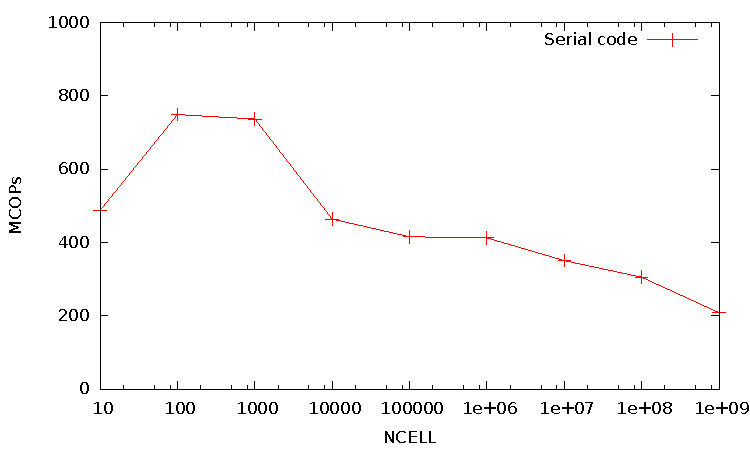
\includegraphics{serialscale}}
\caption{Simple gnuplot example: performance of traffic model}
\label{fig:gnu}
\end{center}
\end{figure}

You can produce the PDF version of Figure~\ref{fig:gnu} from the file
\texttt{serialscale.gp} using \texttt{gnuplot serialscale.gp}.

\section{Conclusions}

This is the place to put your conclusions about your work. You can
split it into different subsections if appropriate. You may want to include
a subsection of future work which could be carried out to continue your
research.

\begin{thebibliography}{100}

\bibitem{ref:lam} L.Lamport. {\em 1986 Latex User's Guide
and Reference Manual.} Addison Wesley. pp242.

\bibitem{ref:bloggs} F.Bloggs. {\em 1993 Latex Users do it
in Environments} Int. Journal of Silly Findings. pp 23-29.

\end{thebibliography}


\end{document}

